%  LaTeX support: latex@mdpi.com 
%  For support, please attach all files needed for compiling as well as the log file, and specify your operating system, LaTeX version, and LaTeX editor.

%=================================================================
\documentclass[journal,article,submit,pdftex,moreauthors]{Definitions/mdpi} 

%--------------------
% Class Options:
%--------------------
%----------
% journal
%----------
% Choose between the following MDPI journals:
% acoustics, actuators, addictions, admsci, adolescents, aerobiology, aerospace, agriculture, agriengineering, agrochemicals, agronomy, ai, air, algorithms, allergies, alloys, analytica, analytics, anatomia, animals, antibiotics, antibodies, antioxidants, applbiosci, appliedchem, appliedmath, applmech, applmicrobiol, applnano, applsci, aquacj, architecture, arm, arthropoda, arts, asc, asi, astronomy, atmosphere, atoms, audiolres, automation, axioms, bacteria, batteries, bdcc, behavsci, beverages, biochem, bioengineering, biologics, biology, biomass, biomechanics, biomed, biomedicines, biomedinformatics, biomimetics, biomolecules, biophysica, biosensors, biotech, birds, bloods, blsf, brainsci, breath, buildings, businesses, cancers, carbon, cardiogenetics, catalysts, cells, ceramics, challenges, chemengineering, chemistry, chemosensors, chemproc, children, chips, cimb, civileng, cleantechnol, climate, clinpract, clockssleep, cmd, coasts, coatings, colloids, colorants, commodities, compounds, computation, computers, condensedmatter, conservation, constrmater, cosmetics, covid, crops, cryptography, crystals, csmf, ctn, curroncol, cyber, dairy, data, ddc, dentistry, dermato, dermatopathology, designs, devices, diabetology, diagnostics, dietetics, digital, disabilities, diseases, diversity, dna, drones, dynamics, earth, ebj, ecologies, econometrics, economies, education, ejihpe, electricity, electrochem, electronicmat, electronics, encyclopedia, endocrines, energies, eng, engproc, entomology, entropy, environments, environsciproc, epidemiologia, epigenomes, est, fermentation, fibers, fintech, fire, fishes, fluids, foods, forecasting, forensicsci, forests, foundations, fractalfract, fuels, future, futureinternet, futurepharmacol, futurephys, futuretransp, galaxies, games, gases, gastroent, gastrointestdisord, gels, genealogy, genes, geographies, geohazards, geomatics, geosciences, geotechnics, geriatrics, grasses, gucdd, hazardousmatters, healthcare, hearts, hemato, hematolrep, heritage, higheredu, highthroughput, histories, horticulturae, hospitals, humanities, humans, hydrobiology, hydrogen, hydrology, hygiene, idr, ijerph, ijfs, ijgi, ijms, ijns, ijpb, ijtm, ijtpp, ime, immuno, informatics, information, infrastructures, inorganics, insects, instruments, inventions, iot, j, jal, jcdd, jcm, jcp, jcs, jcto, jdb, jeta, jfb, jfmk, jimaging, jintelligence, jlpea, jmmp, jmp, jmse, jne, jnt, jof, joitmc, jor, journalmedia, jox, jpm, jrfm, jsan, jtaer, jvd, jzbg, kidneydial, kinasesphosphatases, knowledge, land, languages, laws, life, liquids, literature, livers, logics, logistics, lubricants, lymphatics, machines, macromol, magnetism, magnetochemistry, make, marinedrugs, materials, materproc, mathematics, mca, measurements, medicina, medicines, medsci, membranes, merits, metabolites, metals, meteorology, methane, metrology, micro, microarrays, microbiolres, micromachines, microorganisms, microplastics, minerals, mining, modelling, molbank, molecules, mps, msf, mti, muscles, nanoenergyadv, nanomanufacturing,\gdef\@continuouspages{yes}} nanomaterials, ncrna, ndt, network, neuroglia, neurolint, neurosci, nitrogen, notspecified, %%nri, nursrep, nutraceuticals, nutrients, obesities, oceans, ohbm, onco, %oncopathology, optics, oral, organics, organoids, osteology, oxygen, parasites, parasitologia, particles, pathogens, pathophysiology, pediatrrep, pharmaceuticals, pharmaceutics, pharmacoepidemiology,\gdef\@ISSN{2813-0618}\gdef\@continuous pharmacy, philosophies, photochem, photonics, phycology, physchem, physics, physiologia, plants, plasma, platforms, pollutants, polymers, polysaccharides, poultry, powders, preprints, proceedings, processes, prosthesis, proteomes, psf, psych, psychiatryint, psychoactives, publications, quantumrep, quaternary, qubs, radiation, reactions, receptors, recycling, regeneration, religions, remotesensing, reports, reprodmed, resources, rheumato, risks, robotics, ruminants, safety, sci, scipharm, sclerosis, seeds, sensors, separations, sexes, signals, sinusitis, skins, smartcities, sna, societies, socsci, software, soilsystems, solar, solids, spectroscj, sports, standards, stats, std, stresses, surfaces, surgeries, suschem, sustainability, symmetry, synbio, systems, targets, taxonomy, technologies, telecom, test, textiles, thalassrep, thermo, tomography, tourismhosp, toxics, toxins, transplantology, transportation, traumacare, traumas, tropicalmed, universe, urbansci, uro, vaccines, vehicles, venereology, vetsci, vibration, virtualworlds, viruses, vision, waste, water, wem, wevj, wind, women, world, youth, zoonoticdis 
% For posting an early version of this manuscript as a preprint, you may use "preprints" as the journal. Changing "submit" to "accept" before posting will remove line numbers.

%---------
% article
%---------
% The default type of manuscript is "article", but can be replaced by: 
% abstract, addendum, article, book, bookreview, briefreport, casereport, comment, commentary, communication, conferenceproceedings, correction, conferencereport, entry, expressionofconcern, extendedabstract, datadescriptor, editorial, essay, erratum, hypothesis, interestingimage, obituary, opinion, projectreport, reply, retraction, review, perspective, protocol, shortnote, studyprotocol, systematicreview, supfile, technicalnote, viewpoint, guidelines, registeredreport, tutorial
% supfile = supplementary materials

%----------
% submit
%----------
% The class option "submit" will be changed to "accept" by the Editorial Office when the paper is accepted. This will only make changes to the frontpage (e.g., the logo of the journal will get visible), the headings, and the copyright information. Also, line numbering will be removed. Journal info and pagination for accepted papers will also be assigned by the Editorial Office.

%------------------
% moreauthors
%------------------
% If there is only one author the class option oneauthor should be used. Otherwise use the class option moreauthors.

%---------
% pdftex
%---------
% The option pdftex is for use with pdfLaTeX. Remove "pdftex" for (1) compiling with LaTeX & dvi2pdf (if eps figures are used) or for (2) compiling with XeLaTeX.

%=================================================================
% MDPI internal commands - do not modify
\firstpage{1} 
\makeatletter 
\setcounter{page}{\@firstpage} 
\makeatother
\pubvolume{1}
\issuenum{1}
\articlenumber{0}
\pubyear{2023}
\copyrightyear{2023}
%\externaleditor{Academic Editor: Firstname Lastname}
\datereceived{ } 
\daterevised{ } % Comment out if no revised date
\dateaccepted{ } 
\datepublished{ } 
%\datecorrected{} % For corrected papers: "Corrected: XXX" date in the original paper.
%\dateretracted{} % For corrected papers: "Retracted: XXX" date in the original paper.
\hreflink{https://doi.org/} % If needed use \linebreak
%\doinum{}
%\pdfoutput=1 % Uncommented for upload to arXiv.org

%=================================================================
% Add packages and commands here. The following packages are loaded in our class file: fontenc, inputenc, calc, indentfirst, fancyhdr, graphicx, epstopdf, lastpage, ifthen, float, amsmath, amssymb, lineno, setspace, enumitem, mathpazo, booktabs, titlesec, etoolbox, tabto, xcolor, colortbl, soul, multirow, microtype, tikz, totcount, changepage, attrib, upgreek, array, tabularx, pbox, ragged2e, tocloft, marginnote, marginfix, enotez, amsthm, natbib, hyperref, cleveref, scrextend, url, geometry, newfloat, caption, draftwatermark, seqsplit
% cleveref: load \crefname definitions after \begin{document}

%=================================================================
% Please use the following mathematics environments: Theorem, Lemma, Corollary, Proposition, Characterization, Property, Problem, Example, ExamplesandDefinitions, Hypothesis, Remark, Definition, Notation, Assumption
%% For proofs, please use the proof environment (the amsthm package is loaded by the MDPI class).

%=================================================================
% Full title of the paper (Capitalized)
\Title{An Approach Using Multiple MLP Neural Networks for Predicting the Brazilian Stock Market}

% MDPI internal command: Title for citation in the left column
\TitleCitation{An Approach Using Multiple MLP Neural Networks for Predicting the Brazilian Stock Market}

% Author Orchid ID: enter ID or remove command
\newcommand{\orcidauthorA}{0000-0000-0000-000X} % Add \orcidA{} behind the author's name
%\newcommand{\orcidauthorB}{0000-0000-0000-000X} % Add \orcidB{} behind the author's name

% Authors, for the paper (add full first names)
% \Author{Paulo Tasinaffo $^{1,\dagger,\ddagger}$\orcidA{} and Luiz Dias $^{2,\ddagger}$}
% ORCID of Tasinaffo, P. M.: https://orcid.org/0000-0001-7069-8430
% ORCID of Dias, L. A. V.: https://orcid.org/0000-0002-6544-7458
\Author{Paulo Tasinaffo$^{1}$ and Luiz Dias}

%\longauthorlist{yes}

% MDPI internal command: Authors, for metadata in PDF
\AuthorNames{Paulo Tasinaffo and Luiz Dias}

% MDPI internal command: Authors, for citation in the left column
\AuthorCitation{Tasinaffo, P. M. ; Dias, L. A. V.}
% If this is a Chicago style journal: Lastname, Firstname, Firstname Lastname, and Firstname Lastname.

% Affiliations / Addresses (Add [1] after \address if there is only one affiliation.)
\address{%
$^{1}$ \quad Instituto Tecnológico de Aeronáutica (ITA), São José dos Campos/SP, Brazil; tasinaffo@ita.br}  % \\
% $^{2}$ \quad Affiliation 2; e-mail@e-mail.com}

% Contact information of the corresponding author
% \corres{Correspondence: e-mail@e-mail.com; Tel.: (optional; include country code; if there are multiple corresponding authors, add author initials) +xx-xxxx-xxx-xxxx (F.L.)}

% Current address and/or shared authorship
% \firstnote{Current address: Affiliation 3.} 
% \secondnote{These authors contributed equally to this work.}
% The commands \thirdnote{} till \eighthnote{} are available for further notes

%\simplesumm{} % Simple summary

%\conference{} % An extended version of a conference paper

% Abstract (Do not insert blank lines, i.e. \\) 
\abstract{The Brazilian stock market undergoes many fluctuations over time. This makes him highly unpredictable. To make matters worse, the 2020 pandemic and financial speculation made the Brazilian stock market even more unpredictable. Therefore, in this article, an approach based on Artificial Intelligence is proposed to carry out this prediction. For this purpose, multiple MLP neural networks will be coupled, using supervised learning with input/output training patterns through the NARMAX (Nonlinear Auto Regressive Moving Average with eXogenous input) method. A case study, using the actions of the three main companies in Brazil (PETROBRAS, EMBRAER and Vale do Rio Doce) are considered for the validation of the presented methodology. A numerical and computational comparison between the proposed Multiple method and the method using only one neural network is also presented.}

% Keywords
\keyword{Universal Numerical Integrator (UNI); Nonlinear Auto Regressive Moving Average with eXogenous input (NARMAX); neural differential equations; Euler-Type Universal Numerical Integrator (E-TUNI); Runge-Kutta Neural Network (RKNN); Adams-Bashforth Neural Network (ABNN)} 

% The fields PACS, MSC, and JEL may be left empty or commented out if not applicable
%\PACS{J0101}
%\MSC{}
%\JEL{}

%%%%%%%%%%%%%%%%%%%%%%%%%%%%%%%%%%%%%%%%%%
% Only for the journal Diversity
%\LSID{\url{http://}}

%%%%%%%%%%%%%%%%%%%%%%%%%%%%%%%%%%%%%%%%%%
% Only for the journal Applied Sciences
%\featuredapplication{Authors are encouraged to provide a concise description of the specific application or a potential application of the work. This section is not mandatory.}
%%%%%%%%%%%%%%%%%%%%%%%%%%%%%%%%%%%%%%%%%%

%%%%%%%%%%%%%%%%%%%%%%%%%%%%%%%%%%%%%%%%%%
% Only for the journal Data
%\dataset{DOI number or link to the deposited data set if the data set is published separately. If the data set shall be published as a supplement to this paper, this field will be filled by the journal editors. In this case, please submit the data set as a supplement.}
%\datasetlicense{License under which the data set is made available (CC0, CC-BY, CC-BY-SA, CC-BY-NC, etc.)}

%%%%%%%%%%%%%%%%%%%%%%%%%%%%%%%%%%%%%%%%%%
% Only for the journal Toxins
%\keycontribution{The breakthroughs or highlights of the manuscript. Authors can write one or two sentences to describe the most important part of the paper.}

%%%%%%%%%%%%%%%%%%%%%%%%%%%%%%%%%%%%%%%%%%
% Only for the journal Encyclopedia
%\encyclopediadef{For entry manuscripts only: please provide a brief overview of the entry title instead of an abstract.}

%%%%%%%%%%%%%%%%%%%%%%%%%%%%%%%%%%%%%%%%%%
% Only for the journal Advances in Respiratory Medicine
%\addhighlights{yes}
%\renewcommand{\addhighlights}{%

%\noindent This is an obligatory section in “Advances in Respiratory Medicine”, whose goal is to increase the discoverability and readability of the article via search engines and other scholars. Highlights should not be a copy of the abstract, but a simple text allowing the reader to quickly and simplified find out what the article is about and what can be cited from it. Each of these parts should be devoted up to 2~bullet points.\vspace{3pt}\\
%\textbf{What are the main findings?}
% \begin{itemize}[labelsep=2.5mm,topsep=-3pt]
% \item First bullet.
% \item Second bullet.
% \end{itemize}\vspace{3pt}
%\textbf{What is the implication of the main finding?}
% \begin{itemize}[labelsep=2.5mm,topsep=-3pt]
% \item First bullet.
% \item Second bullet.
% \end{itemize}
%}

%%%%%%%%%%%%%%%%%%%%%%%%%%%%%%%%%%%%%%%%%%
\begin{document}

%%%%%%%%%%%%%%%%%%%%%%%%%%%%%%%%%%%%%%%%%%
% \setcounter{section}{-1} %% Remove this when starting to work on the template.

\section{Introduction}

% \hfill mds
 
% \hfill August 26, 2015

As redes neurais se tornaram muito populares nas últimas décadas, pois são modelos matemáticos complexos e eficientes, que tentam imitar, no computador, o comportamento do cérebro humano. Existem basicamente dois tipos de redes neurais artificiais: redes neurais rasas e redes neurais profundas. As redes neurais rasas foram as maiores contribuições, desta área do conhecimento, durante a última metada do século XX. Por outro lado, as redes neurais profundas são as contribuições mais atuais, sobre o tema, neste século XXI.

Assim sendo, neste artigo é apresentado o modelo NARMAX utilizando Múltiplas Redes Neurais Artificiais (MRNA) com arquitetura Multi-Layer Perceptron (MLP) para a previsão de séries temporais do mercado brasileiro de ações.  A abordagem de treinamento empregada é a aprendizagem supervisionada utilizando padrões de treinamento de entrada/saída. Sendo assim, serão realizados vários experimento computacionais, para verificar se a abordagem proposta, utilizando múltiplas redes neurais, é mais eficiente ou não do que a abordagem utilizando somente uma rede neural artificial.

Este trabalho está dividido em cinco seções. Na Seção 2, é realizada uma revisão bibliográfica das principais referências relacionadas ao tema proposto. Na Seção 3, é desenvolvido o modelo matemático detalhado do algoritmo neural múltiplo proposto. Ainda na Secão 3, uma descrição detalhada do funcionamento da bolsa de valores do mercado brasileiro é também apresentada. Na Seção 4, experimentos computacionais, baseados em dados do mundo real, comparam o desempenho do modelo proposto com aquele obtido com apenas uma rede neural. Por fim, a Seção 5 apresenta as principais conclusões do trabalho proposto.  

\section{Related Works}

Em \cite{ref1} e \cite{ref2}, é demonstrado, formalmente, que as redes neurais Multi-Layer Perceptrons (MLP) com uma camada interna são aproximadores universais de funções. Isto significa que elas podem, pelo menos teoricamente, resolver qualquer problema importante em Inteligência Artificial (e.g., previsão de séries temporais, neurocontrol, diagnóstico médico, classificação de padrões, processamento de imagens, entre outros). Em \cite{ref3}, um resumo das principais arquiteturas neurais rasas do século XX são discutidas em certa profundidade. 

Entretanto, entre todas as possíveis aplicações de redes neurais artificiais, neste artigo, é considerado somente o problema de previsão de séries temporais. Nesta caso, a rede neural artificial pode ser vista como um modelo empírico de equações diferencias autônomas e não-lineares \cite{ref4}. Ainda em \cite{ref4}, é realizada uma classificação dos sistemas dinâmicos tratáveis, através de redes neurais artificiais, que utilizam a abordagem de aprendizagem supervisionada através de padrões de treinamento de entrada/saída. Segundo estes autores, são de três tipos as metodologias para modelagem empírica de sistemas dinâmicos não-lineares, a saber:(i) método NARMAX (Auto Regressive Moving Average with eXogenous input) \cite{ref5} and \cite{ref6}, (ii) metodologia das derivadas médias \cite{ref7, ref8}, and \cite{ref9}, and (iii) metodologia das derivadas instantâneas \cite{ref10, ref11, ref12, ref13}, and \cite{ref14}. Uma visão geral, da utilização de redes neurais artificias e lógica fuzzy, na modelagem de sistemas dinâmicos e posterior aplicação em controle, pode também ver encontrado em \cite{ref15}.

Sendo assim, este artigo pretende realizar a simulação do mercado brasileiro de ações, através do método NARMAX, utilizando múltiplas redes neurais artificiais com arquitetura MLP. O algoritmo de treinamento que será utilizado, nos exemplos apresentados aqui, será o algoritmo Levenberg Marquardt \cite{ref16} de 1994 e que está disponível no Toolbox de Redes Neurais Artificais (ANN) do Matlab.
         

\section{Mathematical Development}

A Seção 3 vai aqui.

Aqui vem o texto 3: \cite{ref1},\cite{ref2}, \cite{ref3}, \cite{ref4}, \cite{ref5}, \cite{ref6}, \cite{ref7}, \cite{ref8}, \cite{ref9}, \cite{ref10}, \cite{ref11}, \cite{ref12}, \cite{ref13}, \cite{ref14}, \cite{ref15} e \cite{ref16}.

O desenvolvimento matemático vai aqui.

\subsection{Relationship Between the Universal Numerical Integrator (UNI) and the NARMAX Model}

A Seção 3.1 vai aqui.

 \begin{figure}[htb]
	\centering
	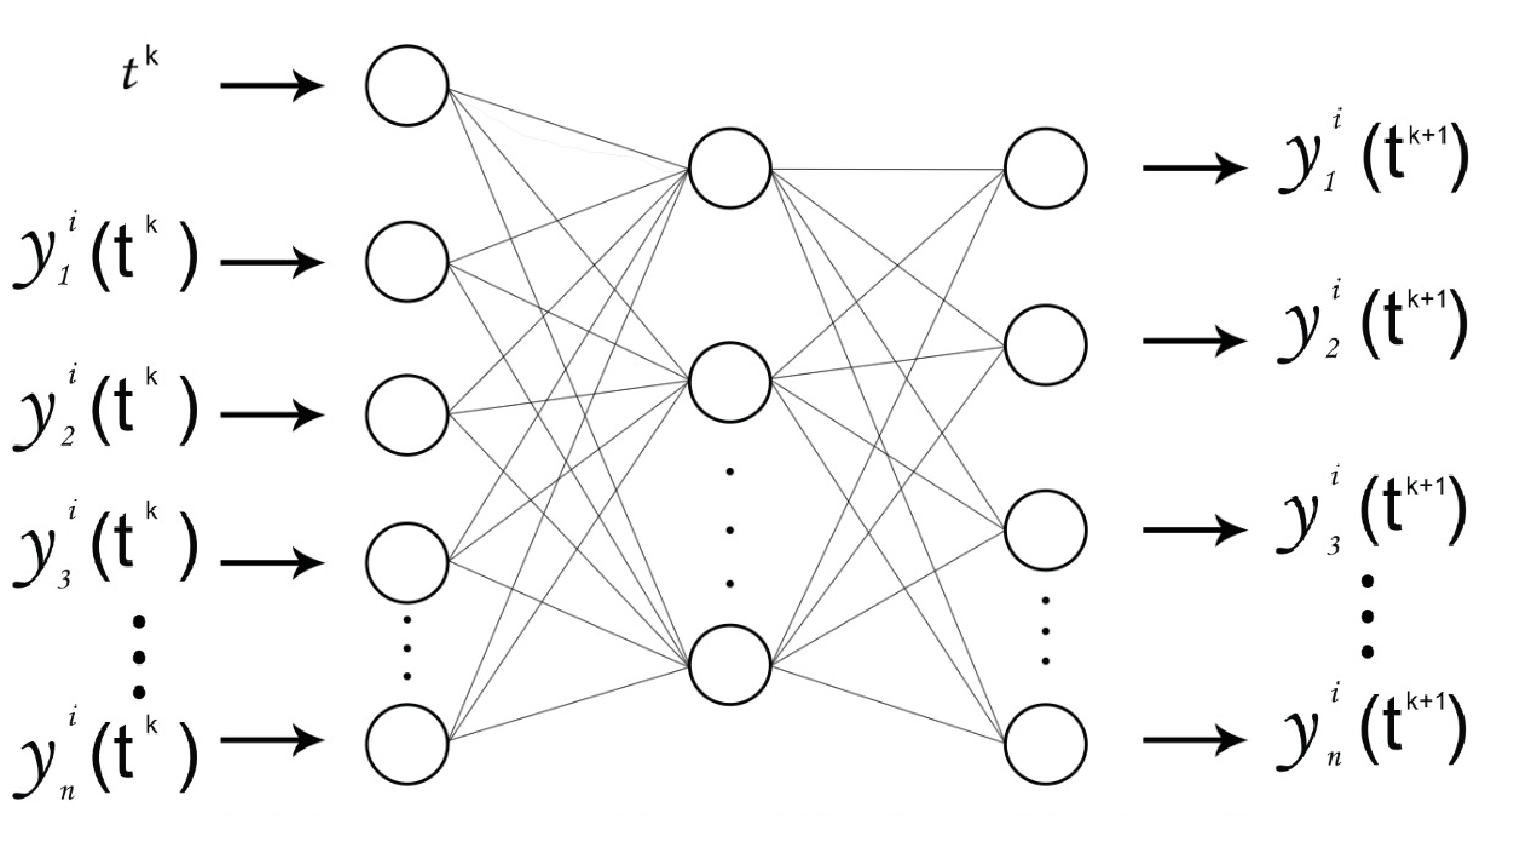
\includegraphics[scale=0.35]{Definitions/figure1.png}
	\caption{Esquema básico da metodologia NARMAX projetada numa arquitetura neural feed-forward (Source: see \cite{ref5, ref6}).}	
	\label{fig1}
\end{figure}

\begin{figure}[htb]
	\centering
	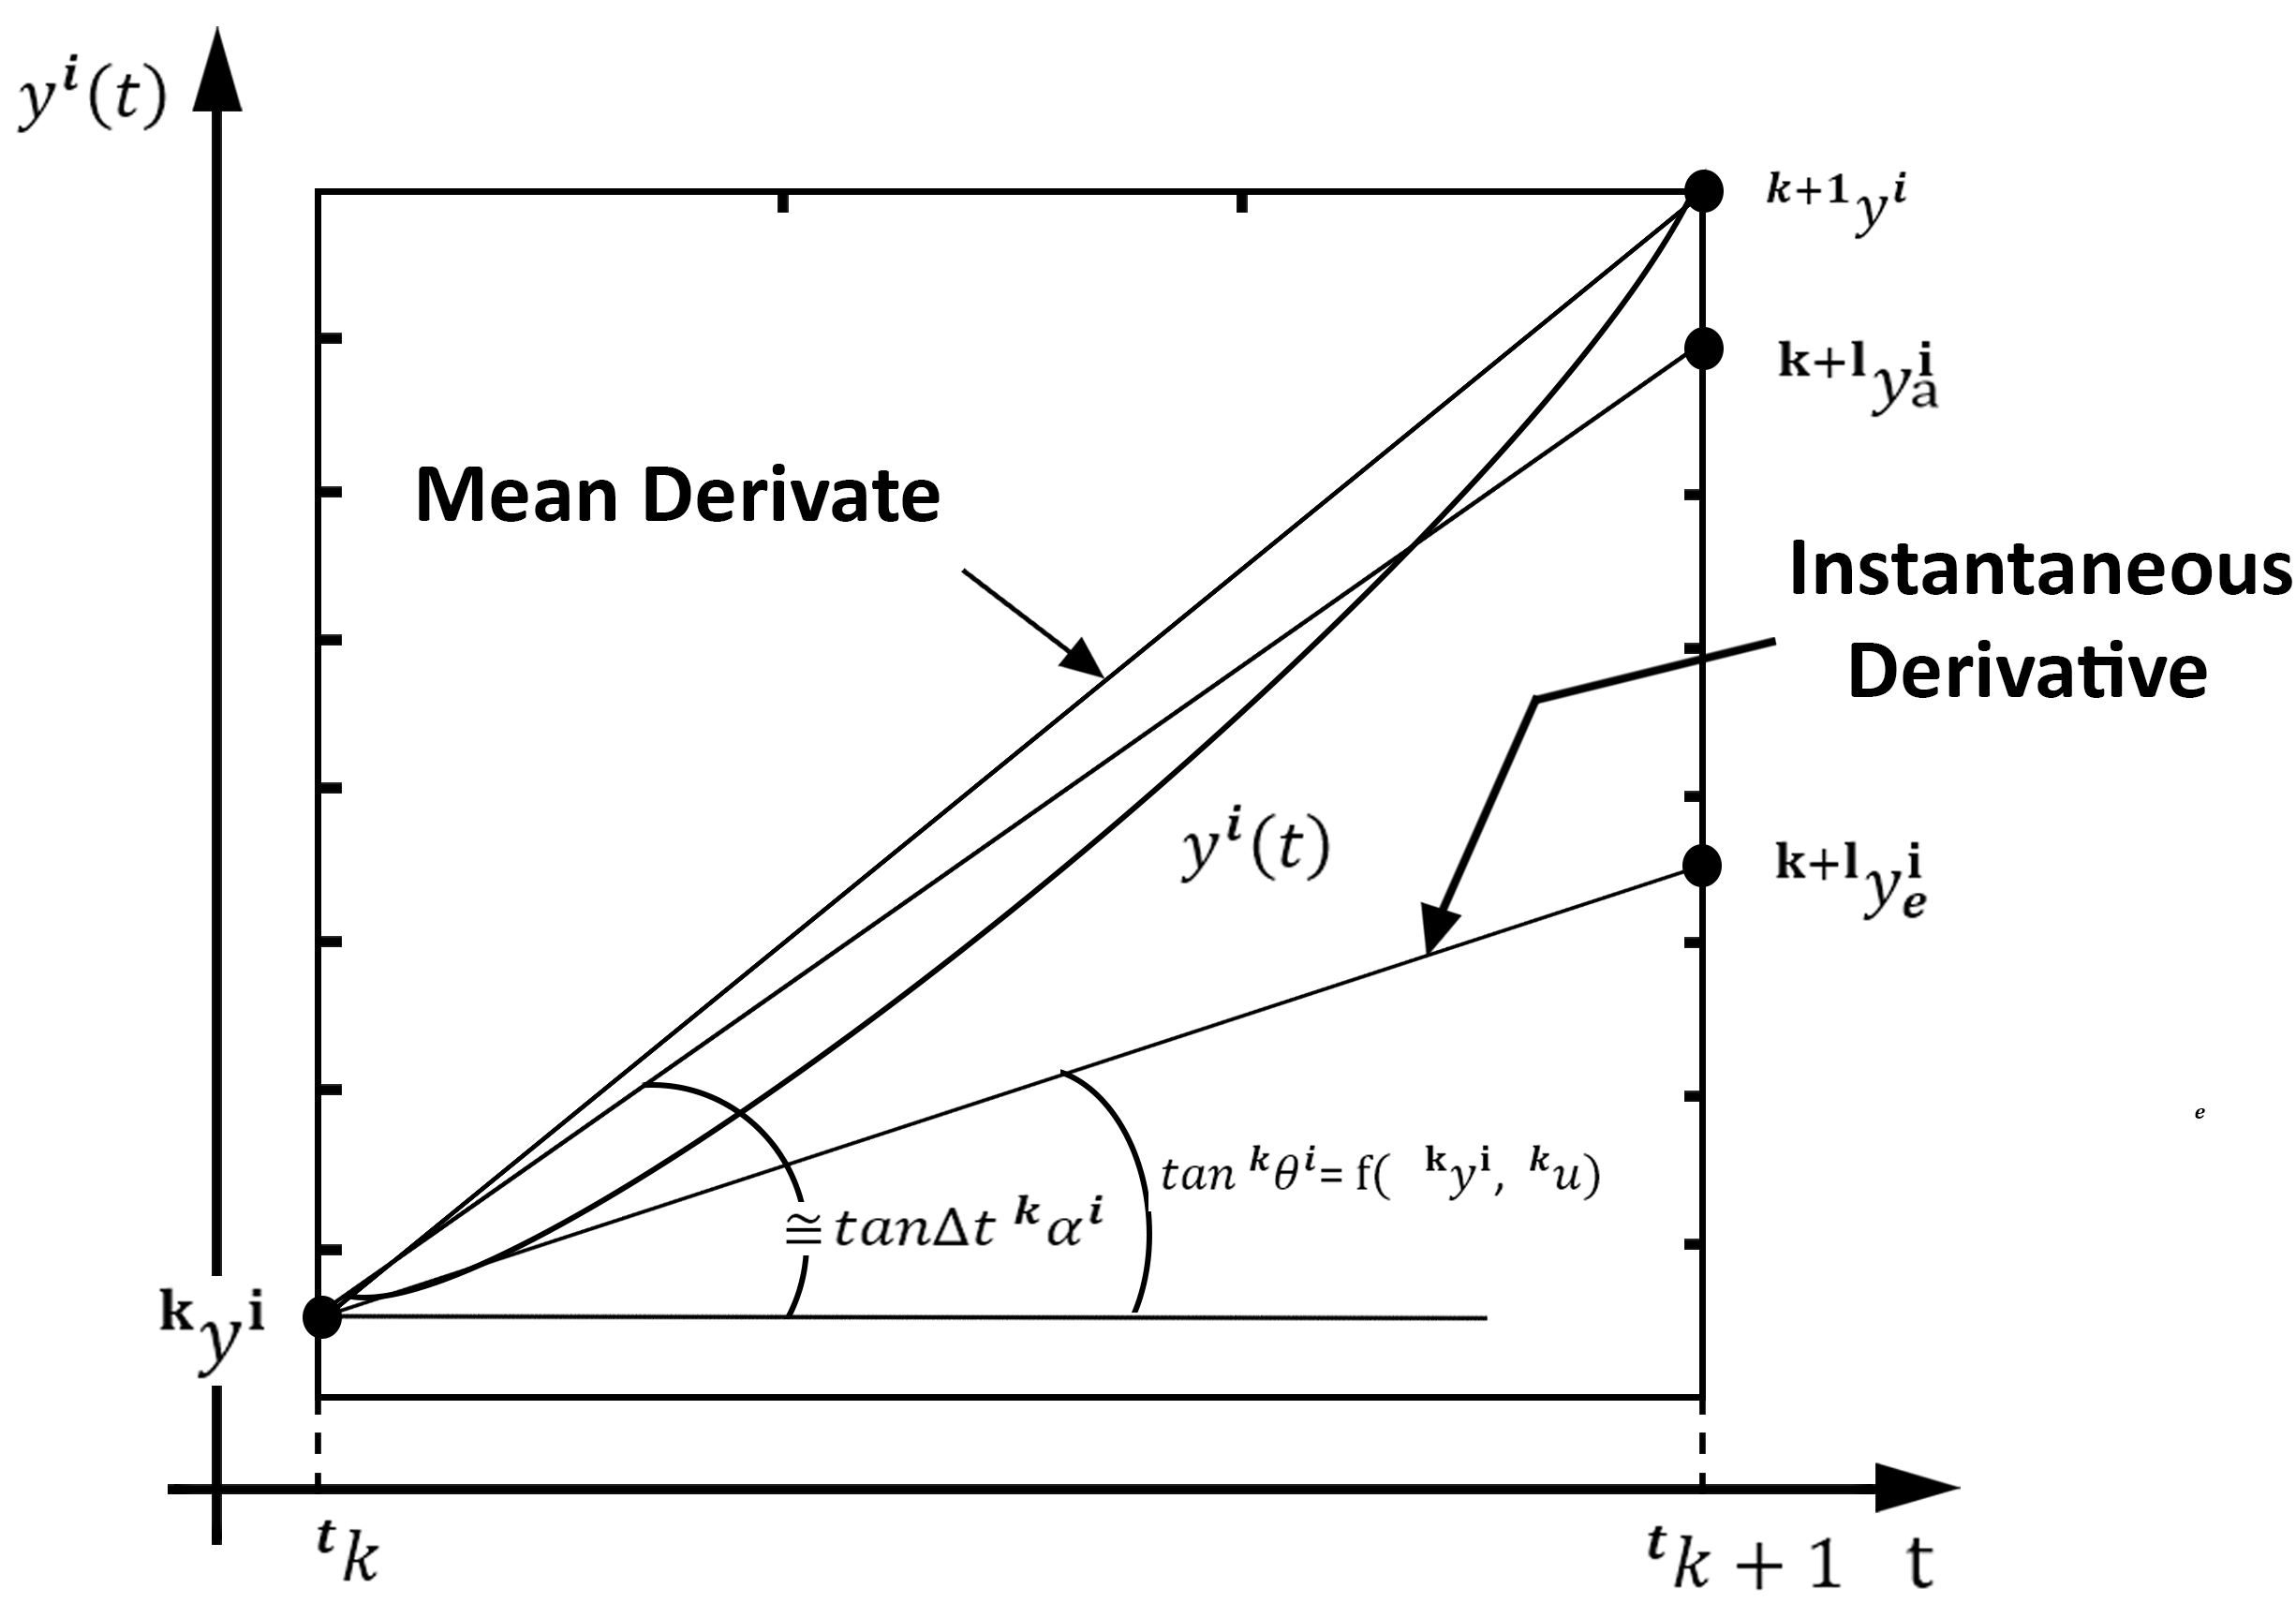
\includegraphics[scale=0.17]{Definitions/figure2.png}
	\caption{Difference between mean derivative and instantaneous derivative functions (Source: see \cite{ref7, ref8}).}
	\label{fig2}
\end{figure}

\begin{figure}[htb]
\centering
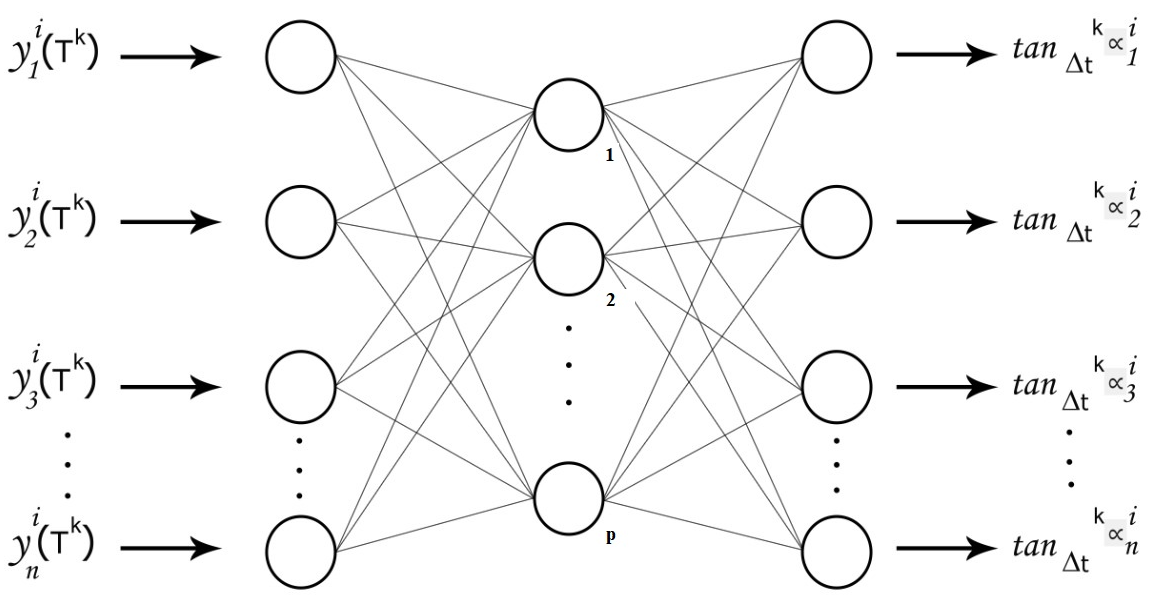
\includegraphics[scale=0.46]{Definitions/figure3.png}
\caption{A feed-forward neural network project with the concept of mean derivative functions.}
\label{fig3}
\end{figure}

\begin{figure}[htb]
\centering
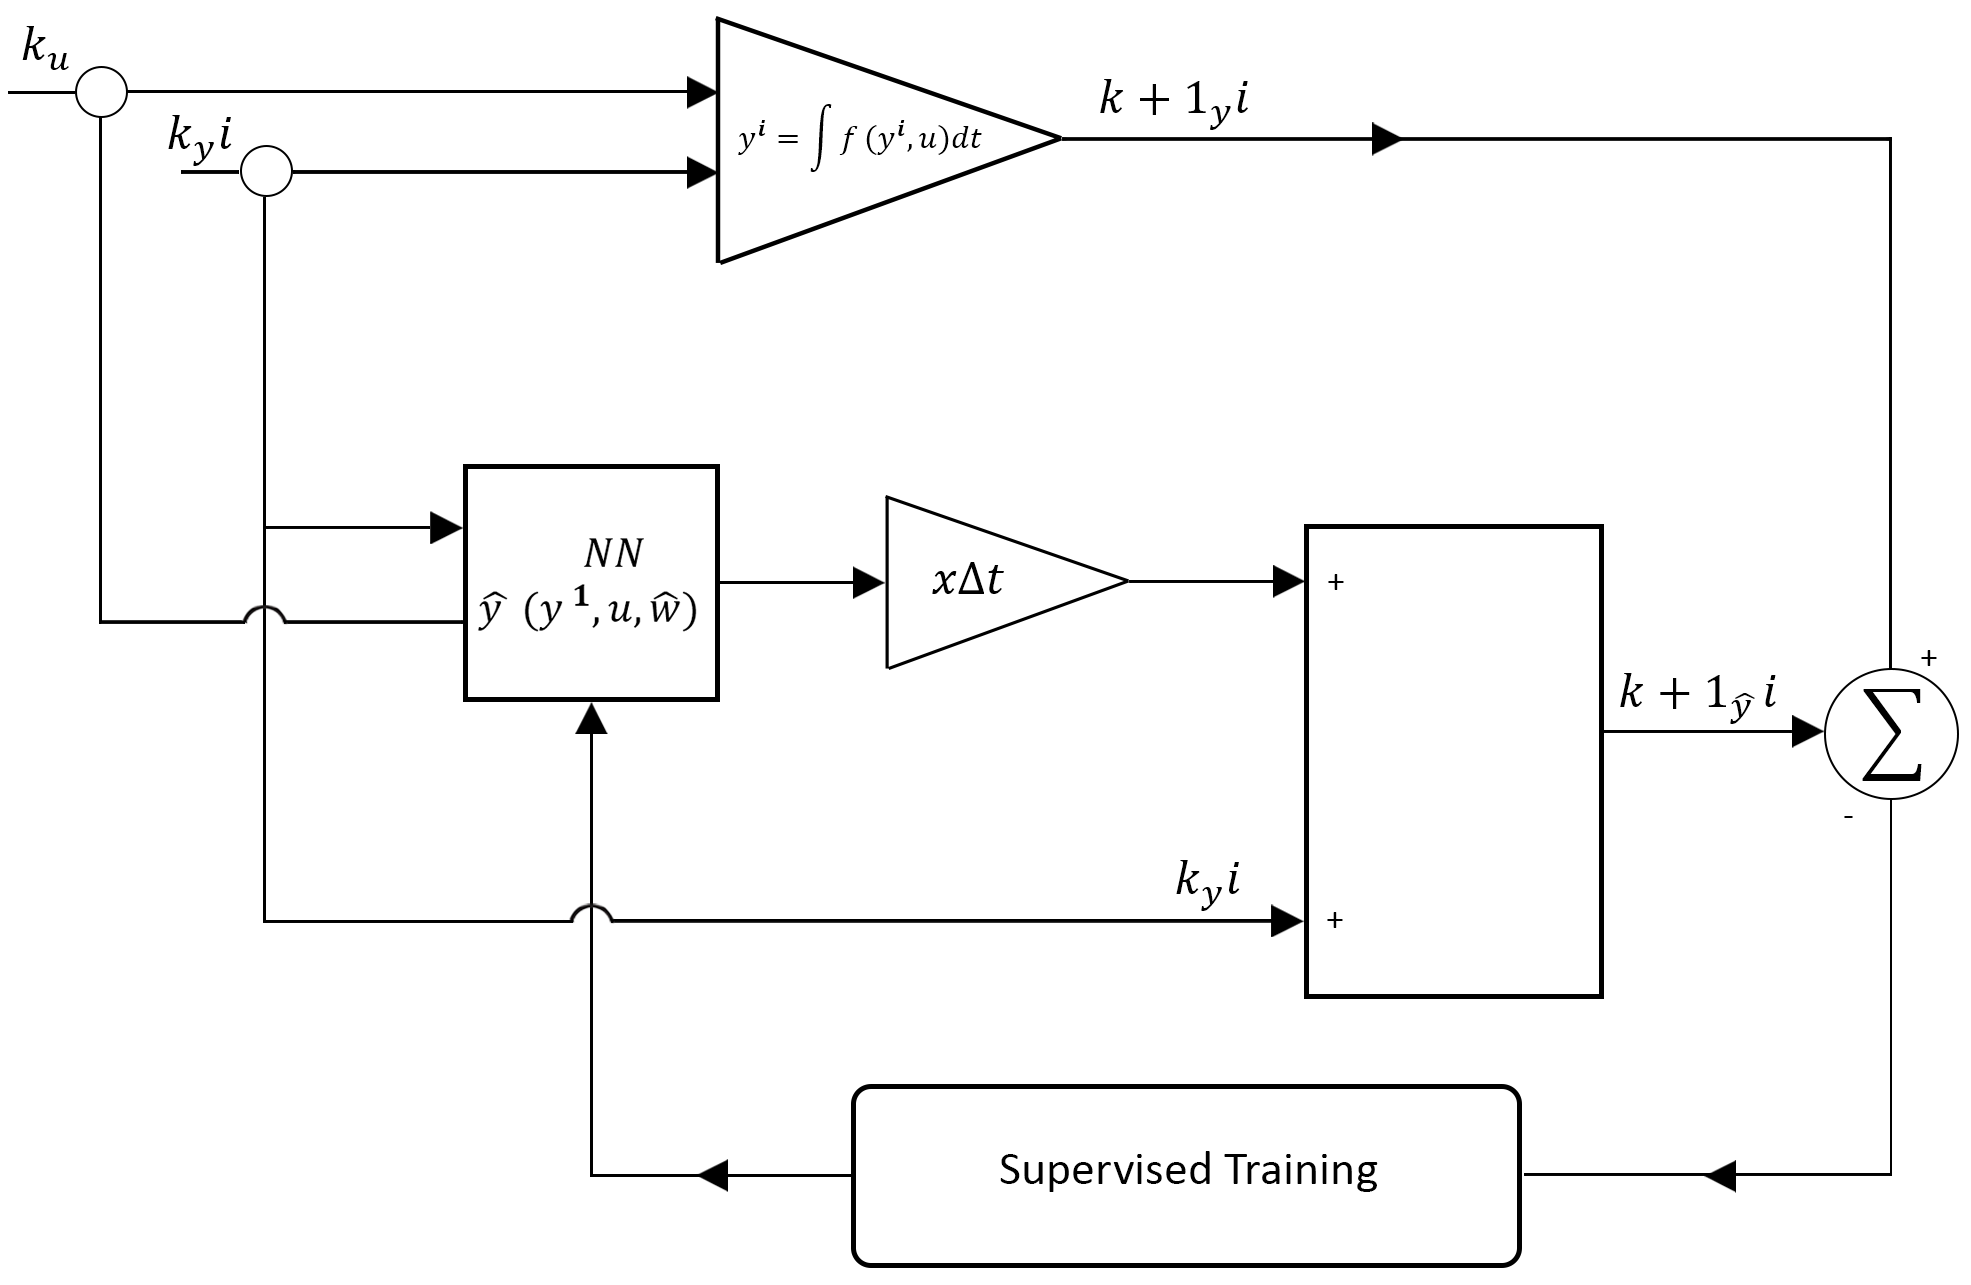
\includegraphics[scale=0.24]{Definitions/figure4.png}
\caption{Esquema básico de uma rede feed-forward projetada internamente no integrador Runge-Kutta 4-5 (Source: see \cite{ref11}).}
\label{fig4}
\end{figure}

\begin{figure}[htb]
\centering
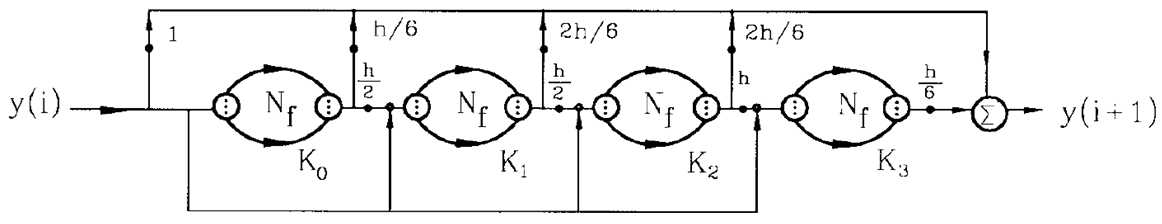
\includegraphics[scale=0.55]{Definitions/figure5.png}
\caption{Esquema básico de uma rede feed-forward projetada internamente no integrador Adams-Bashforth 4 (Source: see \cite{ref12}).}
\label{fig5}
\end{figure}

\begin{equation}
	\left\{\begin{matrix}
		\dot{y}_1= f_1(t, y_1, y_2, \cdots y_n), & y_1(a)=\eta _1 \\
 		\dot{y}_2= f_2(t, y_1, y_2, \cdots y_n), & y_2(a)=\eta _2 \\
 		\vdots & \vdots \\
 		\dot{y}_n= f_n(t, y_1, y_2, \cdots y_n), & y_n(a)=\eta _n 
	\end{matrix}\right.	
	\label{eq:1}
 \end{equation}

Assim, um modelo NARMAX (sem entrada com ruído) do tipo Single-Input e Single-Output (SISO) é dado por \cite{ref5, ref6}:

$$ \hat{y}(k+1)=H[\varphi (k)]= $$
\begin{equation}
	\hat{f}_{NN}
	\begin{bmatrix} y(k) & \cdots & y(k-n_y) & u(k) & \cdots & u(k-n_u)
	\end{bmatrix}
	\label{eq:2}
\end{equation}

Ademais, o modelo NARMAX também pode ser facilmente estendido para o caso Multiple-Input e Multiple-Output (MIMO). Por exemplo, se $ \vec{y}(k-i)= $ $ [y_1(k-i) $ $ y_2(k-i) $ $ \cdots $ $ y_n(k-i)]^T $ e $ \vec{u}(k-j )= $ $ [u_1(k-j) $ $ u_2(k-j) $ $ \cdots $ $ u_n(k-j)]^T $ então,  ter-se-ía o seguinte:

\begin{center}
	$ [\hat{\vec{y}}(k+1) $ $ \hat{\vec{y}}(k+2) $ $ \cdots $ $ \hat{\vec{y}}(k+n_{y_{out }})]= $
\end{center}
%\begin{center} 
% 	$\hat{f}_{NN}[$ $ \vec{y}(k) $ $ \vec{y}(k-1) $ $ \cdots $ $ \vec{y}(k-n_{y_{in}}) $ 
%\end{center}
\begin{equation}
	\hat{f}_{NN}[\quad \vec{y}(k) \quad \vec{y}(k-1) \quad \cdots \quad \vec{y}(k-n_{y_{in}}) \quad  
	\begin{matrix}
		\vec{u}(k) & \vec{u}(k-1) & \cdots & \vec{u}(k-n_{u})
	\end{matrix}]^T
	\label{eq:3}
\end{equation}

Existem também a metodologia das derivadas médias, que é uma alternativa ao modelo NARMAX \cite{ref7, ref8, ref9}. Este tipo de integrador acopla uma rede neural feed-forward ao integrador de Euler de primeira ordem e como esquematizado pelas equações (\ref{eq:4}) e (\ref{eq:5}).

\begin{equation}
{^{k + 1}y^i} = tan_{\Delta t} {^{k}\alpha^i} \cdot \Delta t + {^{k}y^i}
\label{eq:4}
\end{equation}

\noindent onde $ {^{k + 1}y^i}= $ $ [ $ $ {^{k + 1}y_1^i} $ $ {^{k + 2}y_2^i} $ $ \cdots $ $ {^{k + 1}y_n^i} $ $ ]^T $, $ tan_{\Delta t} {^{k + 1} \alpha^i}= $ $ [ $ $ tan_{\Delta t} {^{k + 1} \alpha_1^i} $ $ tan_{\Delta t} {^{k + 1} \alpha_2^i} $ $ \cdots $ $ tan_{\Delta t} {^{k + 1 } \alpha_n^i} $ $ ]^T$ and $ {^{k }y^i}= $ $ [ $ $ {^{k}y_1^i} $ $ {^{k}y_2^i} $ $ \cdots $ $ {^{k}y_n^i} $ $ ]^T $.

\begin{equation}
   tan_{\Delta t} {^{k}\alpha_j^i} = \frac{{^{k+1}y_j^i}-{^{k}y_j^i}}{\Delta t}
\label{eq:5}
\end{equation}

A única Rede Neural Runge-Kutta (RKNN) que está disponível na literatura é a de ordem 4-5 \cite{ref11}:

\begin{equation}
	y_{n+1}= y_n + \frac{h}{6}\cdot(k_1+ 2 \cdot k_2 + 2 \cdot k_3 + k_4)
	\label{eq:6}
\end{equation}

\noindent where,
$$ k_1= N_f(y_n;w) $$
$$ k_2= N_f(y_n + \frac{h}{2}\cdot k_1;w) $$
$$ k_3= N_f(y_n + \frac{h}{2}\cdot k_2;w) $$
$$ k_3= N_f(t_n + h, y_n +{h}\cdot k_3;w) $$
$$ N_f( \cdot, \cdot ;w) \cong \dot{y}=f(y(t))$$

Alternativamente, existe também a Rede Neural Adams-Bashforth (ABNN) que também está disponível na literatura e é dada por \cite{ref12}:
\begin{equation}
	y(t_{n+1})=y(t_n)+ \frac{h}{24} \cdot (55 \cdot f_{n} - 59 \cdot f_{n-1} + 37 \cdot f_{n -2} - 9 \cdot f_{n-3})
	\label{eq:7}
\end{equation}

\subsection{Detailed Description of the Brazilian Financial Stock Market}

Aqui vai a Seção 3.2.


\subsection{Methodology Using Only One MLP Neural Network}


Aqui vai a Seção 3.3.



\subsection{The Proposed Method Using Multiple Neural Networks with MLP Architecture}

Aqui vai a Seção 3.4.



\section{Results and Analysis}

Aqui vai a Seção de Resultados e Experimentos.

\subsection{Simple Method}

Aqui vai a Seção 4.1.

\subsection{Compound Method}

Aqui vai a Seção 4.2.

\subsection{Numerical and Computational Comparisons Between the Two Proposed Methodologies}

Aqui vai a Seção 4.3.

\section{Conclusion}

Aqui vai a Conclusão.



% Paulo Marcelo Tasinaffo está citando \cite{ref1, ref2, ref3, ref4, ref5, ref6, ref7, ref8, ref9, ref10, ref11, ref12, ref13, ref14, ref15, ref16, ref17, ref18, ref19, ref20, ref21, ref22, ref23, ref24, ref25, ref26, ref27, ref28, ref29, ref30, ref31, ref32, ref33, ref34, ref35, ref36, ref37, ref38, ref39, ref40}.

%%%%%%%%%%%%%%%%%%%%%%%%%%%%%%%%%%%%%%%%%%
\vspace{6pt} 

%%%%%%%%%%%%%%%%%%%%%%%%%%%%%%%%%%%%%%%%%%
%% optional
%\supplementary{The following supporting information can be downloaded at:  \linksupplementary{s1}, Figure S1: title; Table S1: title; Video S1: title.}

% Only for journal Methods and Protocols:
% If you wish to submit a video article, please do so with any other supplementary material.
% \supplementary{The following supporting information can be downloaded at: \linksupplementary{s1}, Figure S1: title; Table S1: title; Video S1: title. A supporting video article is available at doi: link.}

% Only for journal Hardware:
% If you wish to submit a video article, please do so with any other supplementary material.
% \supplementary{The following supporting information can be downloaded at: \linksupplementary{s1}, Figure S1: title; Table S1: title; Video S1: title.\vspace{6pt}\\
%\begin{tabularx}{\textwidth}{lll}
%\toprule
%\textbf{Name} & \textbf{Type} & \textbf{Description} \\
%\midrule
%S1 & Python script (.py) & Script of python source code used in XX \\
%S2 & Text (.txt) & Script of modelling code used to make Figure X \\
%S3 & Text (.txt) & Raw data from experiment X \\
%S4 & Video (.mp4) & Video demonstrating the hardware in use \\
%... & ... & ... \\
%\bottomrule
%\end{tabularx}
%}

%%%%%%%%%%%%%%%%%%%%%%%%%%%%%%%%%%%%%%%%%%

\authorcontributions{Methodology, software, and writing was made by P. T.; supervision and project administration, L. D. All authors have read and agree to the published version of the manuscript.}

\funding{The authors thank the Brazilian Aeronautics Institute of Technology (Instituto Tecnológico de Aeronáutica - ITA); the Casimiro Montenegro Filho Foundation (Fundação Casimiro Montenegro Filho - FCMF); and the Brazilian Enterprise Ecossistema Negócios Digitais Ltda for their support and infrastructure, which motivate the challenges and innovations of this research project.}

\institutionalreview{Not applicable.}

\informedconsent{Not applicable.}

\dataavailability{Not applicable.} 

% Only for journal Nursing Reports
%\publicinvolvement{Please describe how the public (patients, consumers, carers) were involved in the research. Consider reporting against the GRIPP2 (Guidance for Reporting Involvement of Patients and the Public) checklist. If the public were not involved in any aspect of the research add: ``No public involvement in any aspect of this research''.}

% Only for journal Nursing Reports
%\guidelinesstandards{Please add a statement indicating which reporting guideline was used when drafting the report. For example, ``This manuscript was drafted against the XXX (the full name of reporting guidelines and citation) for XXX (type of research) research''. A complete list of reporting guidelines can be accessed via the equator network: \url{https://www.equator-network.org/}.}

\acknowledgments{I would like to thank Professors and great friends Atair Rios Neto and Adilson Marques da Cunha for their valuable tips for improving this article. Finally, I would also like to thank the valuable improvement tips given by the good reviewers of this journal. The authors of this article would also like to thank God for making all of this possible.}

\conflictsofinterest{The authors declare no conflict of interest.} 

%%%%%%%%%%%%%%%%%%%%%%%%%%%%%%%%%%%%%%%%%%
%% Optional
% \sampleavailability{Samples of the compounds ... are available from the authors.}

%% Only for journal Encyclopedia
%\entrylink{The Link to this entry published on the encyclopedia platform.}

\abbreviations{Abbreviations}{
The following abbreviations are used in this manuscript:\\

\noindent 
\begin{tabular}{@{}ll}
ABNN     &  Adams-Bashforth Neural Network\\
E-TUNI   &  Euler-Type Universal Numerical Integrator\\
NARMAX   &  Nonlinear Auto Regressive Moving Average with eXogenous input\\
MLP      &  Multi-Layer Perceptron\\
PCNN     &  Predictive-Corrector Neural Network\\
RBF      &  Radial Basis Function\\
RKNN     &  Runge-Kutta Neural Network\\
SVM      &  Support Vector Machine\\  
UNI      &  Universal Numerical Integrator
\end{tabular}
}

%%%%%%%%%%%%%%%%%%%%%%%%%%%%%%%%%%%%%%%%%%
\begin{adjustwidth}{-\extralength}{0cm}
%\printendnotes[custom] % Un-comment to print a list of endnotes

\reftitle{References}

% Please provide either the correct journal abbreviation (e.g. according to the “List of Title Word Abbreviations” http://www.issn.org/services/online-services/access-to-the-ltwa/) or the full name of the journal.
% Citations and References in Supplementary files are permitted provided that they also appear in the reference list here. 

%=====================================
% References, variant A: external bibliography
%=====================================
%\bibliography{your_external_BibTeX_file}

%=====================================
% References, variant B: internal bibliography
%=====================================
\begin{thebibliography}{999}

% Reference 1
\bibitem[Author1(year)]{ref1}
Cybenko, G. \textit{Continuous Valued Networks with Two Hidden Layers Are Sufficient}. University of Illinois at Urbana-Champaign: Center for Supercomputing Research and Development, 1988.

% Reference 2
\bibitem[Author2(year)]{ref2}
Hornik, K.; Stinchcombe, M.; White, H. Multilayer feedforward networks are universal approximators. {\em Neural Networks} {\bf 1989}, {\em 2(5)}, 359--366.

% Reference 3
\bibitem[Author3(year)]{ref3}
Haykin, S. \textit{Neural Networks: A Comprehensive Foundation}. Publisher: Prentice-Hall, Inc., New Jersey, USA, 1999.

% Reference 4
\bibitem[Author4(year)]{ref4}
Tasinaffo, P. M.; Gonçalves, G. S.; Cunha, A. M.; Dias, L. A. V. An introduction to universal numerical integrators. {\em Int. J. Innov. Comput. Inf. Control} {\bf 2019}, {\em 15(1)}, 383--406.

% Reference 5
\bibitem[Author5(year)]{ref5}
Billings, S. A.; Chen, S.; Koreberg, M. J. Identification of {MIMO} non-linear systems using forward-regression orthogonal estimator. {\em Int. J. Control} {\bf 1989}, {\em 49(6)}, 2157--2189.

% Reference 6
\bibitem[Author6(year)]{ref6}
Chen, S. and Billings; S. A. Neural networks for nonlinear dynamic system modelling and identification. {\em Int. J. Control} {\bf 1992}, {\em 56(2)}, 319--346.

% Reference 7
\bibitem[Author7(year)]{ref7}
Tasinaffo, P. M. Estruturas de Integração Neural Feedforward Testadas em Problemas de Controle Preditivo. Doctoral Thesis, INPE-10475-TDI/945, São José dos Campos/SP, Brazil, 2003.

% Reference 8
\bibitem[Author8(year)]{ref8}
Tasinaffo, P. M.; Rios Neto, A. Mean derivatives based neural {E}uler integrator for nonlinear dynamic systems modeling. {\em Learning and Nonlinear Models} {\bf 2005}, {\em 3(2)}, 98--109.

% Reference 9
\bibitem[Author9(year)]{ref9}
de Figueiredo, M. O.; Tasinaffo, P. M.; Dias, L. A. V. Modeling autonomous nonlinear dynamic systems using mean derivatives, fuzzy logic and genetic algorithms. {\em Int. J. Innov. Comput. Inf. Control} {\bf 2016}, {\em 12(5)}, 1721--1743.


% Reference 10
\bibitem[Author10(year)]{ref10}
Vidyasagar, M. \textit{Nonlinear Systems Analysis}. Publisher: Prentice-Hall, Inc., Electrical Engineering Series, New Jersey, USA, 1978.

% Reference 11
\bibitem[Author11(year)]{ref11}
Wang, Y.-J.; Lin, C.-T. Runge-{K}utta neural network for identification of dynamical systems in high accuracy. {\em IEEE Transactions on Neural Networks} {\bf 1998}, {\em 9(2)}, 294--307.

% Reference 12
\bibitem[Author12(year)]{ref12}
Tasinaffo, P. M.; Rios Neto, A. Adams-{B}ashforth neural networks applied in a predictive control structure with only one horizon. {\em Int. J. Innov. Comput. Inf. Control} {\bf 2019}, {\em 15(2)}, 445--464.

% Reference 13
\bibitem[Author13(year)]{ref13}
Chen, R. T. Q.; Rubanova, Y.; Bettencourt, J.; Duveand, D. Neural ordinary differential equations. In Proceedings of the 32nd Conference on Neural Information Processing Systems (NeurlPS), Montréal, Canada, 2018, 1--19.

% Reference 14
\bibitem[Author14(year)]{ref14}
Uçak, K. A {R}unge-{K}utta {MLP} neural network based control method for nonlinear {MIMO} systems. In Proceedings of the 6th International Conference on Electrical and Electronics Engineering (ICEEE), Istanbul, Turkey, 2019, 186-192.

% Reference 15
\bibitem[Author15(year)]{ref15}
Spooner, J. T.; Maggiore, M.; Ordónez, R.; Passino, K. M. \textit{Stable Adaptive Control and Estimation for Nonlinear Systems Neural and Fuzzy Approximator Techniques}. Publisher: Wiley-Interscience, New York, USA, 2002.

% Reference 16
\bibitem[Author16(year)]{ref16}
Hagan, M. T.; Menhaj, M. B Training feedforward networks with the Marquardt algorithm. {\em IEEE Transactions on Neural Networks} {\bf 1994}, {\em 5(6)}, 989--993.


% Reference 6
%\bibitem[Author6(year)]{ref6}
%Hornik, K.; Stinchcombe, M.; White, H. Multilayer feedforward networks are universal approximators. {\em Neural Networks} {\bf 1989}, {\em 2(5)}, 359--366.

% Reference 7
%\bibitem[Author7(year)]{ref7}
%Haykin, S. \textit{Neural Networks: A Comprehensive Foundation}. Publisher: Prentice-Hall, Inc., New Jersey, USA, 1999.

% Reference 8
%\bibitem[Author8(year)]{ref8}
%Author 1, A.B.; Author 2, C.D.; Author 3, E.F. Title of presentation. In Proceedings of the Name of the Conference, Location of Conference, Country, Date of Conference (Day Month Year); Abstract Number (optional), Pagination (optional).

% Reference 9
%\bibitem[Author9(year)]{ref9}
%Author 1, A.B. Title of Thesis. Level of Thesis, Degree-Granting University, Location of University, Date of Completion.

\end{thebibliography}

% If authors have biography, please use the format below
%\section*{Short Biography of Authors}
%\bio
%{\raisebox{-0.35cm}{\includegraphics[width=3.5cm,height=5.3cm,clip,keepaspectratio]{Definitions/author1.pdf}}}
%{\textbf{Firstname Lastname} Biography of first author}
%
%\bio
%{\raisebox{-0.35cm}{\includegraphics[width=3.5cm,height=5.3cm,clip,keepaspectratio]{Definitions/author2.jpg}}}
%{\textbf{Firstname Lastname} Biography of second author}

% For the MDPI journals use author-date citation, please follow the formatting guidelines on http://www.mdpi.com/authors/references
% To cite two works by the same author: \citeauthor{ref-journal-1a} (\citeyear{ref-journal-1a}, \citeyear{ref-journal-1b}). This produces: Whittaker (1967, 1975)
% To cite two works by the same author with specific pages: \citeauthor{ref-journal-3a} (\citeyear{ref-journal-3a}, p. 328; \citeyear{ref-journal-3b}, p.475). This produces: Wong (1999, p. 328; 2000, p. 475)

%%%%%%%%%%%%%%%%%%%%%%%%%%%%%%%%%%%%%%%%%%
%% for journal Sci
%\reviewreports{\\
%Reviewer 1 comments and authors’ response\\
%Reviewer 2 comments and authors’ response\\
%Reviewer 3 comments and authors’ response
%}
%%%%%%%%%%%%%%%%%%%%%%%%%%%%%%%%%%%%%%%%%%
\PublishersNote{}
\end{adjustwidth}
\end{document}

